\documentclass{article}

\usepackage{PRIMEarxiv}

\usepackage[utf8]{inputenc} % allow utf-8 input
\usepackage[T1]{fontenc}    % use 8-bit T1 fonts
\usepackage{hyperref}       % hyperlinks
\usepackage{url}            % simple URL typesetting
\usepackage{booktabs}       % professional-quality tables
\usepackage{amsfonts}       % blackboard math symbols
\usepackage{amsmath}
\usepackage{nicefrac}       % compact symbols for 1/2, etc.
\usepackage{microtype}      % microtypography
\usepackage{fancyhdr}       % header
\usepackage{graphicx}       % graphics
\usepackage{multirow}
\usepackage{xcolor}
\usepackage{enumitem}
\graphicspath{{media/}}     % organize your images and other figures under media/ folder
\setlist{itemsep=1pt,topsep=2pt}

\newcommand{\pmci}[1]{\,{\scriptsize$\pm$#1}}
\newcommand{\yes}{\textbf{supported}}
\newcommand{\no}{\textbf{not supported}}

%Header
\pagestyle{fancy}
\thispagestyle{empty}
\rhead{ \textit{ }}

% Update your Headers here
\fancyhead[LO]{Structure, Information and Inference in 5-a-Side Football}

%% Title
\title{Structure, Information and Inference in 5-a-Side Football:\\
Can Formations Compensate for Limited Vision?
}

\author{
  Arpan Gupta \\
  IIT Gandhinagar \\
  Gandhinagar \\
  \texttt{24110051@iitgn.ac.in} \\
  \And
  Deep Buha \\
  IIT Gandhinagar \\
  Gandhinagar \\
  \texttt{24110082@iitgn.ac.in} \\
  \And
  Ramji Purwar \\
  IIT Gandhinagar \\
  Gandhinagar \\
  \texttt{ramji.purwar@iitgn.ac.in} \\
}


\begin{document}
\maketitle


\begin{abstract}
We study cooperative multi-agent reinforcement learning in a 5-a-side football game without goalkeepers, in which
every player sees opponents only within a limited radius. Our team is one parameter-shared MAPPO policy; the opponent is
a hand-written zonal team that holds a formation. Around one theme, \emph{structure versus information}, we ask three
questions and answer each with trained teams, held-out test matches and 95\% confidence intervals. \textbf{(Q1)} Giving
the team a formation does \emph{not} measurably help at any radius: pooled over radii the formation spot changes the win
score by $+0.09\pm0.15$ and an enforced formation by $-0.12\pm0.16$, while the training seed alone moves one setting from
$W=0.18$ to $0.76$. A single seed per setting would have produced a confident but false $+0.42$ benefit.
\textbf{(Q2)} A formation change by the opponent can be identified from what the players see within about 30 steps
(2.5\% of a match) by a Bayesian filter; handing over to a specialist on that guess keeps 97\% of the oracle's gain
(regret $0.01\pm0.04$). Teams trained end to end on the switch did not learn to identify it: they learned one
policy that beats both formations. \textbf{(Q3)} An opponent ``playmaker'' costs the unaware team 0.54--0.80 in win score.
Identify-then-act wins back 2--47\% of that cost and stays below an oracle (12--81\%); a single recurrent team trained
on all cases, warm-started from a trained team, does best of all (0.70 against 0.35 and 0.42 over the seven playmaker
cases, paired over the same 3{,}500 matches). In total we trained 65 teams (about 2.5 million training matches,
$3\times10^9$ game steps). The common thread is that learned robustness beat both structure and explicit inference,
and that seed variance, not structure, dominates small-budget comparisons.
\end{abstract}


% keywords can be removed
\keywords{Multi-agent reinforcement learning \and Football \and Partial observability \and Formations \and
Opponent modelling \and Bayesian filtering}


%====================================================================================================================
\section{Introduction}
\label{sec:intro}

Team sports are everyday examples of multi-agent decision making under partial information. No player sees the whole
pitch, teammates coordinate without constant communication, and opponents change tactics during a match. Human teams
cope in two ways: they rely on \emph{structure}, a formation that tells every player where to be by default, and they
gather \emph{information}, by looking around and working out what the opponent is doing. The same ingredients
(partial observation, cooperation, changing adversaries) appear in robot soccer~\cite{kitano1997robocup}, in
Google Research Football~\cite{kurach2020grf,song2023grf} and in multi-robot coordination.

We built a minimal 2D 5-a-side game in which these two resources can be varied independently, trained teams with
parameter-shared MAPPO~\cite{yu2022mappo}, and asked three questions (as in our proposal):

\begin{enumerate}[leftmargin=2.2em]
\item[\textbf{Q1}] \textbf{Structure versus vision.} Can a formation compensate for limited vision? Does its benefit
grow as the vision radius shrinks, and does the best formation depend on the radius?
\item[\textbf{Q2}] \textbf{Inference.} If the opponent switches formation mid-match without telling us, how quickly can our
team infer it from partial observations, and how much is inferring it worth? We compare an explicit Bayesian filter, an
oracle, and recurrent (GRU) and memoryless (MLP) teams trained end to end.
\item[\textbf{Q3}] \textbf{Adapting to a playmaker.} If one opponent is a playmaker with full-pitch vision, can our team
work out who it is and adapt? How much of the lost win score does an adaptive team recover, compared with an unaware
team and an oracle that is told who the playmaker is?
\end{enumerate}

\paragraph{Summary of findings.} Table~\ref{tab:summary} gives the answers. Every number in this paper comes from the
result files of the runs (Appendix~\ref{app:repro}); $W$ is the win score (wins plus half the draws) on held-out test
matches, and $\pm$ is a 95\% interval.

\begin{table}[h]
\caption{The three questions and our answers.}
\label{tab:summary}
\centering
\small
\begin{tabular}{p{0.25\linewidth}p{0.69\linewidth}}
\toprule
Question & Answer (Section) \\
\midrule
\textbf{Q1.} Can a formation compensate for limited vision? &
\textbf{No, not measurably} (\S\ref{sec:q1}). Formation as information: $+0.09\pm0.15$; enforced formation:
$-0.12\pm0.16$ (pooled over radii, 33 runs). No evidence that the benefit grows as vision shrinks, and the best
formation does not measurably depend on the radius. The training seed matters more than structure. Learned teams
cope with limited vision far better than the hand-written team (at 12\,m: $W$ 0.45--0.61 against 0.07). \\
\textbf{Q2.} How fast can a formation switch be inferred, and what is it worth? &
\textbf{In about 30 steps, almost for free} (\S\ref{sec:q2}). A Bayesian filter finds the switch in a median 28
steps at $r=25$ and keeps 97\% of the oracle's gain (regret $0.01\pm0.04$); at $r=12$ regret is $0.07\pm0.06$.
End-to-end training learns robustness instead of identification, and memory (GRU) did not help over an MLP. \\
\textbf{Q3.} Can the team identify and neutralise a playmaker? &
\textbf{Partly} (\S\ref{sec:q3}). The playmaker costs the unaware team 0.54--0.80. It is identified from behaviour
in 99--100\% of matches in three of four cases, after 140--195 steps. Identify-then-act recovers 2--47\% of the cost,
below the oracle (12--81\%). A single recurrent team trained on all cases recovers the most (53--81\%). \\
\bottomrule
\end{tabular}
\end{table}

\paragraph{Contributions.} (i) A small, fast 5v5 environment with formations, three structure levels, radius-limited
vision, a formation-holding zonal opponent that can switch formation, and an optional playmaker. (ii) A controlled
multi-seed measurement of the structure benefit across vision radii (46 Q1 runs). (iii) A comparison of explicit
Bayesian identification, an oracle and end-to-end recurrent/memoryless training for a hidden formation switch, with
detection delay, adaptation lag and regret. (iv) A playmaker study with cost, recovery $\kappa$, regret, identification
accuracy and delay, and a test of whether the adaptive teams actually mark the playmaker. (v) A quantified case study of
how much seed variance can mislead single-seed comparisons in MARL~\cite{henderson2018matters,agarwal2021precipice}.

\paragraph{Organisation.} Section~\ref{sec:prelim} introduces the notation and definitions, Section~\ref{sec:problem}
states the three questions formally, Section~\ref{sec:setup} describes what we built and gives the results for Q1--Q3,
Sections~\ref{sec:discussion}--\ref{sec:conclusion} discuss them, and Section~\ref{sec:contrib} lists the tasks of each
member. Appendix~\ref{app:changes} lists every change from our proposal.

\subsection{Related work}
\label{sec:related}

\textbf{Football as a MARL testbed.} RoboCup~\cite{kitano1997robocup} established football as an AI benchmark, and
Google Research Football~\cite{kurach2020grf} is the standard 3D-physics RL environment; Song et
al.~\cite{song2023grf} survey MARL on it. Those environments are expensive per match; ours trades physical detail for
speed, so that we could train dozens of seeds per question.
\textbf{Partial observability.} Our problem is a Dec-POMDP~\cite{bernstein2002complexity,oliehoek2016concise}. Beliefs
over hidden state~\cite{kaelbling1998pomdp} motivate our explicit filters; recurrent policies with GRUs~\cite{cho2014gru}
are the standard learned alternative.
\textbf{Learning.} We use PPO~\cite{schulman2017ppo} with GAE~\cite{schulman2016gae} under centralised training and
decentralised execution~\cite{lowe2017maddpg}, in the MAPPO form of Yu et al.~\cite{yu2022mappo}. Our reward uses
potential-based shaping, which leaves the optimal policy unchanged~\cite{ng1999shaping}, also with several
learners~\cite{devlin2011shaping}.
\textbf{Opponent modelling.} Identifying a hidden opponent type and best-responding to it is a classic opponent-modelling
setting~\cite{albrecht2018modelling}; Q2 and Q3 compare this identify-then-act design with end-to-end training.
\textbf{Evaluation.} Deep RL results vary strongly across seeds~\cite{henderson2018matters}, and point estimates from few
runs mislead~\cite{agarwal2021precipice}. We report intervals over training seeds throughout and only claim
differences whose 95\% interval excludes zero.

%====================================================================================================================
\section{Preliminaries}
\label{sec:prelim}

\subsection{Notation}
Table~\ref{tab:notation} lists the symbols used in the rest of the paper. The numeric values are those of the final
implementation.

\begin{table}[h]
\caption{Notation.}
\label{tab:notation}
\centering
\small
\begin{tabular}{ll}
\toprule
Symbol & Meaning \\
\midrule
$\mathcal N,\mathcal M$ (each $\{1,\dots,5\}$) & players of our team; players of the opponent \\
$t\in\{0,\dots,T\}$, $T=1{,}200$ & time step; length of a match \\
$\mathcal P=[0,100]\times[0,60]$\,m & the pitch \\
$x_i^t,\;y_j^t,\;b^t\in\mathcal P$ & position of our player $i$, of opponent $j$, of the ball \\
$\psi^t\in\{\text{ours},\text{theirs},\text{loose}\}$ & possession \\
$\mathcal F$, $\alpha_f(k)$ & formations \{2-2-1, 2-1-2, 1-3-1, 1-2-2, 3-1-1\}; anchor (home spot) of slot $k$ in $f$ \\
$f$;\; $g^t\in\mathcal F$ & our formation (fixed); opponent formation at step $t$ (hidden from us) \\
$\mathcal G$ & opponent formation process (fixed, drawn per match, or switching) \\
$\zeta\in\{0,1,2\}$ & structure level of our team \\
$r$;\; $\rho_j$ & vision radius of our players; of opponent $j$ ($25$\,m, or $\infty$ for a playmaker) \\
$\sigma\in\{0,\dots,5\}$ & index of the opponent playmaker ($0$: none), hidden from us \\
$C=(f,\zeta,\mathcal G,\sigma,r)$ & match configuration \\
$o_i^t$, $h_i^t$, $a_i^t$ & observation, history and action of our player $i$ \\
$\pi_\theta$, $\hat\theta$ & shared policy; parameters returned by training \\
$\Phi$, $\gamma$ & shaping potential; discount ($0.99$) \\
$G_T$ & final goal difference (ours minus theirs) \\
$W(\theta;C)$ & win score (wins plus half the draws) \\
$\mu^t$, $h$, $\beta$ & belief of a filter; switch hazard; evidence exponent \\
\bottomrule
\end{tabular}
\end{table}

\subsection{Decentralised POMDPs and centralised training}
A Dec-POMDP~\cite{bernstein2002complexity,oliehoek2016concise} is a tuple
$\langle\mathcal N,\mathcal S,\{\mathcal A_i\},P,R,\{\Omega_i\},O,\gamma,T\rangle$ with a state space, per-agent
actions, a transition kernel, one shared team reward, per-agent observation spaces with an observation kernel, a
discount and a horizon. The opponent is a fixed program, so we treat it as part of $P$. The history of player $i$ is
$h_i^t=(o_i^0,a_i^0,\dots,o_i^t)$. All our players share one policy $\pi_\theta(a_i^t\mid h_i^t,i)$; the feed-forward (MLP)
version uses only $o_i^t$ (and the previous action), and the recurrent version keeps a hidden state
$z_i^t=\mathrm{GRU}_\theta(z_i^{t-1},o_i^t)$~\cite{cho2014gru}. Under centralised training and decentralised
execution~\cite{lowe2017maddpg,yu2022mappo}, a critic $V_\phi(s^t)$ sees the full state during training only; at play
time each player acts from its own history.

\subsection{Formations, structure levels and control rating}
A formation $f\in\mathcal F$ (named defenders--midfielders--forwards) gives slot $k$ an anchor $\alpha_f(k)$, a home spot
that moves up and down the pitch with possession; our player $i$ occupies slot $k=i$. The structure level $\zeta$ sets
how much of the formation our team is given:
$\zeta=0$, the formation only sets kick-off positions; $\zeta=1$ (structure as information), the player observes its
anchor and has a \textsc{hold\_shape} action, but leaving the anchor costs nothing; $\zeta=2$ (structure as
constraint), as $\zeta=1$, and tackle, pass and shot success are multiplied by the control rating
\begin{equation}
c_\zeta(x,\alpha)=
\begin{cases}
1, & \zeta<2,\\
c_{\min}+(1-c_{\min})\exp\!\left(-\|x-\alpha\|^2/L^2\right), & \zeta=2,
\end{cases}
\qquad c_{\min}=0.5,\;L=20\text{\,m}.
\label{eq:control}
\end{equation}
The opponent always plays with $\zeta=2$.

\subsection{Limited vision}
For a player at $x$ with radius $\rho$, the visibility of a point $z$ is $v(z;x,\rho)=\mathbb 1[\|z-x\|\le\rho]$. Our
players use $\rho=r$. Opponents are observed only when $v=1$; teammates and the ball are always observed (a
simplification of the final game, Appendix~\ref{app:changes}). We write $v_{ij}^t=v(y_j^t;x_i^t,r)$.

\subsection{Potential-based reward shaping}
A shaping term of the form $F(s,s')=\gamma\Phi(s')-\Phi(s)$ for any potential $\Phi$ leaves the set of optimal
policies unchanged~\cite{ng1999shaping}, also when several learners share it~\cite{devlin2011shaping}. It therefore
needs no fading, and a policy cannot gain from it by cycling between states, since the shaping along any cycle sums to
(nearly) zero.

\subsection{Bayesian filtering of a hidden opponent type}
\label{sec:filter}
Let $\mathcal K$ be a finite set of hypotheses about the opponent (its current formation in Q2; ``no playmaker'' or
``opponent $k$ is the playmaker'' in Q3), and $e^t$ what our five players see together at step $t$. A belief
$\mu^t$ over $\mathcal K$ starts uniform and is updated by
\begin{align}
\tilde\mu^t(k)&=(1-h)\,\mu^{t-1}(k)+h\,\frac{1-\mu^{t-1}(k)}{|\mathcal K|-1}, \label{eq:predict}\\
\mu^t(k)&\propto\tilde\mu^t(k)\;P(e^t\mid k)^{\beta}. \label{eq:update}
\end{align}
The hazard $h$ allows the hypothesis to change during a match ($h=0$ when it cannot, as for the playmaker). The
likelihoods $P(e^t\mid k)$ are frequency maps counted on practice matches (Section~\ref{sec:q2}). Consecutive steps
show nearly the same picture, so the evidence is far from independent; the exponent $\beta<1$ discounts it. The guess
is the hypothesis on top of $\mu^t$ (Q2), or the top hypothesis once its probability reaches a commit threshold (Q3).

\subsection{Win score and statistics}
For parameters $\theta$ and configuration $C$, the win score is
\begin{equation}
W(\theta;C)=\Pr[G_T>0]+\tfrac12\Pr[G_T=0],
\label{eq:W}
\end{equation}
over the randomness of the game, the opponent and the policy. A difference of win scores between two teams is an
\emph{effect}. The $W$ of a training setting is the mean over its training seeds, with a 95\% Student-$t$ interval
over seeds; a difference between two settings uses Welch's interval~\cite{welch1947}, which does not assume equal
variances. When fixed teams play the same matches (same match seeds), differences are paired over matches. We call a
difference a finding only if its 95\% interval excludes 0.

%====================================================================================================================
\section{Problem Formulation}
\label{sec:problem}

\subsection{Match model}
A match is played under a configuration $C=(f,\zeta,\mathcal G,\sigma,r)$.

\textbf{State.} $s^t=(x^t_{1:5},\,y^t_{1:5},\,b^t,\,\psi^t,\,g^t,\,\sigma,\,t)$, plus ball flight and short freezes
after failed tackles.

\textbf{Actions.} $a_i^t\in\mathcal A$, $|\mathcal A|=27$: eight walking directions, stay, \textsc{hold\_shape}
(only if $\zeta\ge1$), go to ball, pass to teammate $k$, through ball to teammate $k$, dribble, shoot, tackle, and
\textsc{shadow}$_j$ (move between opponent $j$ and our goal, only if $v_{ij}^t=1$). Invalid actions are masked.

\textbf{Observation.} In the frame of player $i$ (positions relative to $x_i^t$),
\begin{equation}
o_i^t=\Big(x_i^t,\;a_i^{t-1},\;i,\;\{x_k^t\}_{k\ne i},\;\{(y_j^t v_{ij}^t,\,v_{ij}^t)\}_{j\in\mathcal M},\;b^t,\;\psi^t,\;
\alpha_f(i)\,\mathbb 1[\zeta\ge1],\;G_t,\;t/T\Big),
\label{eq:obs}
\end{equation}
where unseen opponents are zeroed and flagged. The opponent formation $g^t$, the way it switches and the playmaker
$\sigma$ are \emph{not} observed (except by the oracles of Q2 and Q3, which are told $g^t$ or $\sigma$).

\textbf{Reward and objective.} The team reward is
\begin{equation}
R^t=100\big(\mathbb 1[\text{goal for us}]-\mathbb 1[\text{goal against}]\big)+\gamma\Phi(s^{t+1})-\Phi(s^t),
\qquad J(\theta;C)=\mathbb E_{\pi_\theta,C}\Big[\textstyle\sum_{t=0}^{T}\gamma^tR^t\Big],
\label{eq:reward}
\end{equation}
with $\Phi(s)=10\,p(b)+30\,q(s)$, where $p(b)\in[-1,1]$ is the ball's position along the pitch ($-1$ at our goal line,
$+1$ at theirs) and $q(s)$ is the current carrier's chance to score if it shot now, positive for us and negative for
them. PPO returns an approximate maximiser $\hat\theta\approx\arg\max_\theta\mathbb E_{C\sim\mathcal D}[J(\theta;C)]$
for a training distribution $\mathcal D$ of configurations, so our conclusions concern trained policies, not exact
optima.

\subsection{Q1: Can formation structure compensate for limited vision?}
Let the opponent formation be fixed within a match ($g^t\equiv g$, drawn per match from
$\mathcal F_{\text{train}}=\{\text{2-2-1, 2-1-2, 1-3-1, 3-1-1}\}$) and $\sigma=0$. For each $(\zeta,f,r)$ let
\begin{gather}
W_\zeta(f,r)=W\big(\hat\theta_\zeta(f,r);(f,\zeta,\mathcal G,0,r)\big),\qquad
B_\zeta(f,r)=W_\zeta(f,r)-W_0(f,r)\;\;(\zeta\in\{1,2\}),\notag\\
f^\star(r)=\arg\max_f W_1(f,r).
\label{eq:q1}
\end{gather}
We ask: (a) is $B_\zeta(f,r)>0$; (b) does $B_\zeta$ decrease as $r$ grows; (c) does $f^\star(r)$ change with $r$; and
(d) is knowing the anchor ($\zeta=1$) different from being bound to it ($\zeta=2$), i.e.\ is $W_2-W_1\ne0$? As a
benchmark, $M(f,g)$ is the win matrix of the scripted team against itself; its best formation on average and its
maximin formation $\arg\max_f\min_g M(f,g)$ are compared with $f^\star(r)$.

\subsection{Q2: Inferring and adapting to a formation change}
\textbf{Switch process.} The opponent starts in $g_0$ and switches to $g_1$ at a hidden time $\tau$:
$g^t=g_0$ for $t<\tau$ and $g_1$ after. We test two processes: \emph{random time},
$\tau\sim\mathcal U\{100,\dots,1100\}$ with $g_0=$ 2-2-1, $g_1=$ 1-2-2; and \emph{on the score}, where every 50 steps
the opponent goes to 1-2-2 if it is behind and to 3-1-1 if it is ahead.

\textbf{Policies.} (1) \emph{keep}: a general policy $\hat\theta_{\text{gen}}$ trained against
$\mathcal F_{\text{train}}$; (2) \emph{oracle}: $\hat\theta_{\text{gen}}$ until $\tau$, then a specialist
$\hat\theta_{g_1}$ trained against $g_1$; (3) \emph{guess} (identify-then-act): the specialist plays while the filter of
Eqs.~\eqref{eq:predict}--\eqref{eq:update} guesses $g_1$; (4) end-to-end recurrent (GRU) and memoryless (MLP) policies
trained on the switch itself, which must handle it implicitly.

\textbf{Measures.} The regret of a policy is $\mathrm{Reg}(\theta)=W(\text{oracle};C)-W(\theta;C)$, paired over
matches. With $\hat g^t$ the filter's guess, the detection delay of a switch is
\begin{equation}
\Delta_{\text{det}}=\min\{t-\tau:\;t\ge\tau,\;\hat g^{t'}=g_1\;\forall t'\in\{t,\dots,t+m-1\}\},
\label{eq:delay}
\end{equation}
with persistence $m$ (undetected switches are censored at the end of the match). The adaptation lag is the number of
steps after $\tau$ until the goal-difference rate, averaged over matches aligned at their own switch, returns to its
pre-switch level. All parameters of the filter are tuned on matches from the training distribution only.

\subsection{Q3: Adapting to an opponent playmaker}
One opponent $\sigma\in\{1,\dots,5\}$ is a playmaker (its vision is $\rho_\sigma=\infty$, with the further abilities of
Section~\ref{sec:q3}); $\sigma$ is hidden. With $\hat\theta_{\text{base}}$ the unaware team (trained with
$\sigma=0$), the cost of the playmaker and the recovery of a team $\theta$ are
\begin{equation}
E(\sigma)=W(\hat\theta_{\text{base}};\sigma{=}0)-W(\hat\theta_{\text{base}};\sigma),\qquad
\kappa(\sigma)=\frac{W(\theta;\sigma)-W(\hat\theta_{\text{base}};\sigma)}{E(\sigma)},
\label{eq:q3}
\end{equation}
where $\kappa=1$ means that all of the cost is won back; $\kappa$ is reported only when the 95\% interval of $E(\sigma)$
excludes 0. The regret of the adaptive team is $\mathrm{Reg}_\sigma=W(\text{oracle};\sigma)-W(\text{adaptive};\sigma)$, and
the value of the shadow action is $A_{\text{sh}}(\sigma)=W(\text{mix};\sigma)-W(\text{mix-no-shadow};\sigma)$. We also
measure how often and how fast the playmaker is identified, and how often our players shadow it.

%====================================================================================================================
\section{Solutions and Results}
\label{sec:setup}

This section first describes what we built and how we trained and evaluated (\S\ref{sec:env}--\ref{sec:protocol}), then
answers Q1--Q3 in turn (\S\ref{sec:q1}--\ref{sec:q3}).

\subsection{Environment and opponent}
\label{sec:env}

\begin{figure}[t]
  \centering
  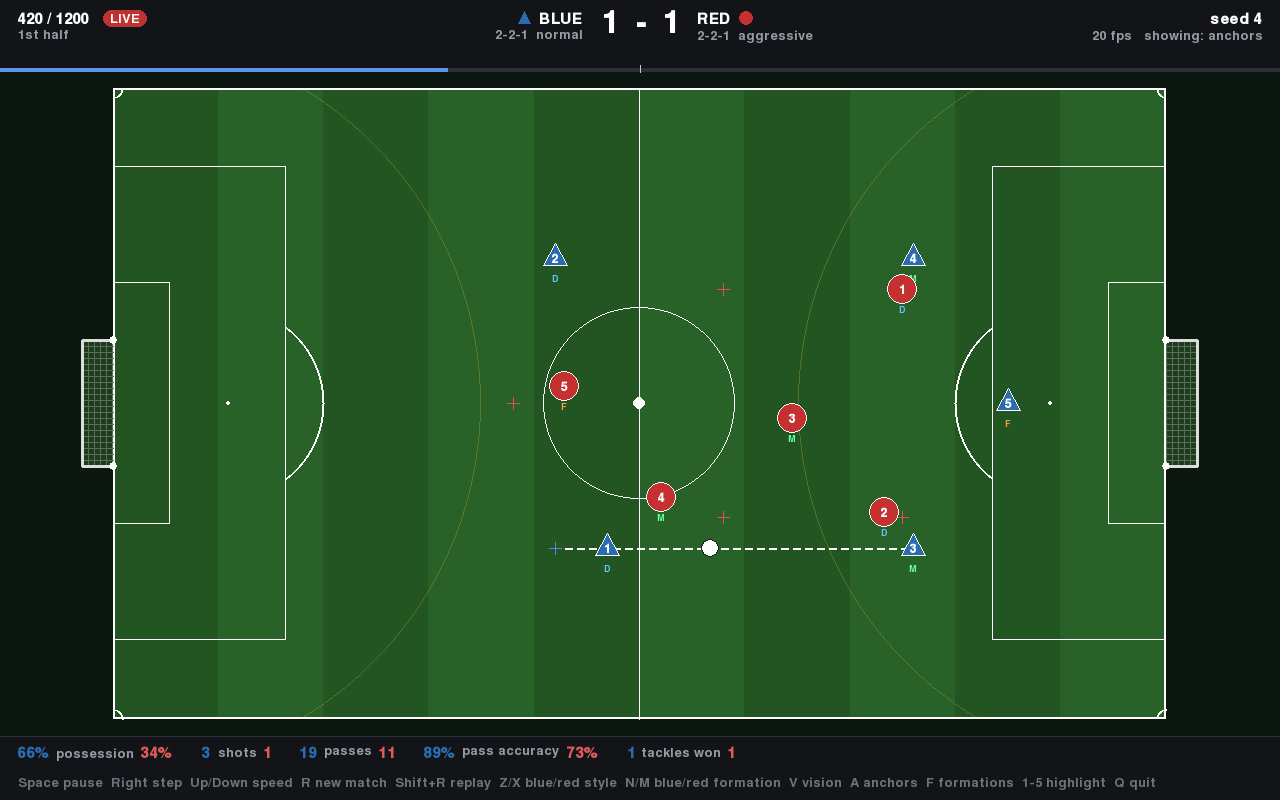
\includegraphics[width=0.82\linewidth]{viewer.png}
  \caption{A moment from a test match in our viewer (blue: our learned team in 2-2-1; red: the scripted opponent).
  The pitch is $100\times60$\,m; a match lasts 1{,}200 steps. Every player sees opponents only within its vision radius.}
  \label{fig:viewer}
\end{figure}

\textbf{The game.} Two teams of five outfield players play on a $100\times60$\,m pitch with 12\,m goals and no
goalkeepers, for $T=1{,}200$ steps (Figure~\ref{fig:viewer}). Every step all ten players act simultaneously. Positions
are continuous and 2D; passes and shots travel along the ground. Passes can be intercepted (a defender takes the ball if
it can reach the ball's path in time), tackles succeed with a probability that falls with distance and fail with a
short freeze, and a shot scores with probability $p = 0.8\,e^{-d/30}\cdot\text{openness}\cdot c$, where $d\le35$\,m is
the distance to goal, openness falls with defenders near the shot line, and $c$ is the shooter's control rating
(Eq.~\ref{eq:control}). More goals after 1{,}200 steps wins; draws count half. We use $r\in\{12, 25, 120\}$\,m, where
120\,m covers the whole pitch (``full vision''). Passes are offered only when no defender \emph{the passer can see}
could reach the ball, so vision still matters: an unseen defender can still intercept.

\textbf{The opponent.} A fixed, hand-written team that does not learn. Each player holds a home spot from the formation;
without the ball the team defends zones (the nearest player presses, one covers, the rest shift towards the ball); with
the ball the carrier shoots, passes forward, carries or lays off, using only what it sees. Because players stay near
their spots, the formation is readable from where they stand (Phase~0 below), which makes Q2 well posed. It can switch
formation mid-match (players walk to their new spots), and one player can be made a playmaker (\S\ref{sec:q3}).

\textbf{Phase 0 checks.} Before training we checked the game with the scripted team on both sides (300 matches per line,
\texttt{runs/phase0/phase0.txt}). (i) A random team loses every match ($W=0.00$, goal difference $-6.5$), and the game
is balanced (scripted vs.\ scripted $W=0.48\pm0.05$). (ii) Vision matters: a scripted team with $r=12$ scores
$W=0.14\pm0.03$ against the same team with $r=25$. (iii) A playmaker with full vision lowers the other side's $W$
from about 0.5 to 0.26--0.36 in every case tried. (iv) The formation win matrix $M(f,g)$ between scripted teams has
1-3-1 as the best formation on average ($\bar W=0.67$) and 1-2-2 as the maximin formation (worst case 0.51).

\subsection{Learning}
\textbf{Algorithm.} Parameter-shared MAPPO~\cite{yu2022mappo} as in \S\ref{sec:prelim}: one actor network is shared by
our five players, each acting on its own observation (Eq.~\ref{eq:obs}); a centralised critic sees the full state during
training only. The actor is an MLP with 256 hidden units, or a GRU~\cite{cho2014gru} of the same width in Q2 and Q3.
PPO~\cite{schulman2017ppo}: $\gamma=0.99$, GAE $\lambda=0.95$~\cite{schulman2016gae}, clip 0.2, 5 epochs, minibatch
1{,}024, learning rates $3\cdot10^{-4}$ (actor) and $10^{-3}$ (critic), entropy coefficient 0.01, value normalisation,
48 games in parallel. The reward is Eq.~\eqref{eq:reward}; its shaping is potential-based, so it is never faded and
cannot be farmed by passing back and forth.

\textbf{Easy start (curriculum).} A new team cannot beat the full-strength opponent, so each opponent player initially
takes a random action with probability $\epsilon=0.5$. $\epsilon$ drops by 0.05 whenever we win 60\% of 50 evaluation
matches and rises when we win 40\% or less.

\textbf{Budget.} Every run trains for 40{,}000 matches (48 million game steps) unless stated. A run took about
13--16 hours on one 40-thread CPU server; seven servers ran one run each in parallel.

\subsection{Evaluation protocol}
\label{sec:protocol}
Every 1{,}000 training matches a checkpoint is saved and evaluated on 50 matches against the full-strength opponent
with fixed seeds. The best checkpoint is then played on \textbf{300 new test matches} whose seeds were never used before;
this \emph{test} $W$ (Eq.~\ref{eq:W}) is what we report. 300 matches give a standard error of about $\pm0.03$ for one
run. Because the seed-to-seed spread is far larger than that, settings are compared over training seeds with the
intervals of \S\ref{sec:prelim}. With one seed we give no interval at all.

%====================================================================================================================
\subsection{Results for Q1: formation structure under limited vision}
\label{sec:q1}

\textbf{Design.} Our team plays 2-2-1 against the scripted opponent, whose formation is drawn per match from 2-2-1,
2-1-2, 1-3-1 and 3-1-1 and is not told to our team (1-2-2, the maximin formation of Phase~0, was held out and later
serves as the Q2 target). For each structure
level $\zeta\in\{0,1,2\}$ and radius $r\in\{12,25,120\}$ we trained 4 seeds ($\zeta=0,1$) or 3 seeds ($\zeta=2$): 33
runs. We also trained our team in 1-3-1 and 1-2-2 at $\zeta=1$ (13 runs; 4 seeds each at 12\,m). The structure benefit
$B_\zeta(r)$ and the best formation $f^\star(r)$ are as in Eq.~\eqref{eq:q1}.

\begin{table}[t]
\caption{Q1 test $W$ (mean over seeds $\pm$ 95\% interval) and the structure benefit with Welch 95\% intervals.
No benefit excludes 0.}
\label{tab:q1}
\centering
\small
\begin{tabular}{lccc}
\toprule
 & $r=12$\,m & $r=25$\,m & full vision \\
\midrule
$\zeta=0$ (no formation), 4 seeds & $0.45\pm0.45$ & $0.76\pm0.18$ & $0.63\pm0.24$ \\
\quad each seed & 0.18, 0.25, 0.62, 0.76 & 0.60, 0.77, 0.84, 0.84 & 0.40, 0.68, 0.70, 0.73 \\
$\zeta=1$ (formation as information), 4 seeds & $0.61\pm0.29$ & $0.82\pm0.16$ & $0.68\pm0.38$ \\
\quad each seed & 0.44, 0.53, 0.60, 0.86 & 0.75, 0.77, 0.78, 0.96 & 0.41, 0.66, 0.67, 0.99 \\
$\zeta=2$ (formation enforced), 3 seeds & $0.52\pm0.33$ & $0.55\pm0.43$ & $0.42\pm0.41$ \\
\quad each seed & 0.39, 0.51, 0.65 & 0.41, 0.49, 0.74 & 0.25, 0.45, 0.58 \\
\midrule
$B_1 = W_1-W_0$ & $+0.16$ [$-0.27$, $+0.59$] & $+0.05$ [$-0.13$, $+0.23$] & $+0.05$ [$-0.31$, $+0.42$] \\
$B_2 = W_2-W_0$ & $+0.07$ [$-0.36$, $+0.49$] & $-0.22$ [$-0.57$, $+0.14$] & $-0.20$ [$-0.54$, $+0.13$] \\
$W_2-W_1$ (cost of enforcing) & $-0.09$ [$-0.40$, $+0.21$] & $-0.27$ [$-0.62$, $+0.09$] & $-0.26$ [$-0.65$, $+0.13$] \\
\midrule
Scripted team in our seat (reference) & 0.07 & 0.45 & 0.54 \\
\bottomrule
\end{tabular}
\end{table}

\begin{figure}[t]
  \centering
  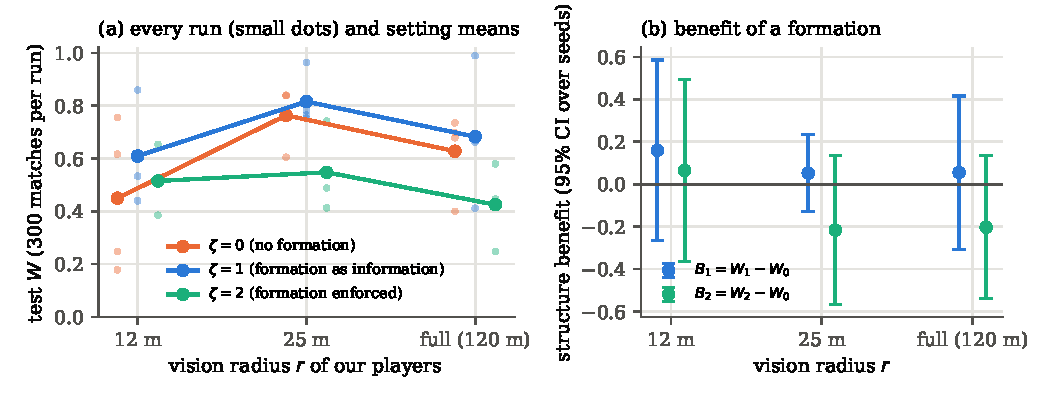
\includegraphics[width=\linewidth]{q1_main.pdf}
  \caption{Q1. (a) Test $W$ of all 33 runs; small dots are individual seeds, lines join setting means. (b) Structure
  benefit $B_\zeta(r)$ with 95\% Welch intervals over seeds. Every interval contains 0.}
  \label{fig:q1}
\end{figure}

\textbf{A formation does not measurably help} (Table~\ref{tab:q1}, Figure~\ref{fig:q1}). Pooled over the three radii
(each radius centred on its own mean), the formation spot changes $W$ by $+0.09\pm0.15$ (12 vs.\ 12 runs) and the
enforced formation by $-0.12\pm0.16$ (9 vs.\ 12 runs). Both intervals include 0. If anything, enforcing the formation
costs a little: at 25\,m and with full vision $\zeta=2$ is the lowest setting, by $-0.27$ and $-0.26$ against $\zeta=1$,
although neither interval excludes 0.

\textbf{The benefit does not grow as vision shrinks.} The point estimates lean towards the hypothesis ($B_1$ is
$+0.16$ at 12\,m against $+0.05$ at 25\,m and full vision), but $B_1(12)-B_1(25)=+0.11$ [$-0.40$, $+0.61$] and
$B_1(12)-B_1(120)=+0.10$ [$-0.50$, $+0.71$]. The hypothesis is not supported.

\textbf{Seed variance dominates.} Without a formation at 12\,m, the four seeds ended at $W=0.18$, 0.25, 0.62 and 0.76.
The spread within a setting is larger than any difference between settings. Had we trained one seed per setting (seed
0 only), we would have reported a clean $B_1(12)=0.60-0.18=+0.42$, an effect the full data do not support. A
play-style analysis of the first 16 runs (100 extra matches each) explains the spread: at 12\,m without a formation,
two seeds learned a deep defence with fast counter-attacks (mean $W$ 0.69) and two drifted into a possession game
(possession 28\% against 10\%, mean $W$ 0.22) that a team seeing only 12\,m cannot make work; across those runs more
possession went with lower $W$ (correlation $-0.51$). The worst $\zeta=1$ seed beats the worst $\zeta=0$ seed at 12\,m
(0.44 against 0.18) and at 25\,m (0.75 against 0.60), but not with full vision (0.41 against 0.40); over all radii the
seed spread is the same with and without the formation (SD 0.17 and 0.18), so this is an observation, not a tested effect.

\begin{figure}[t]
  \centering
  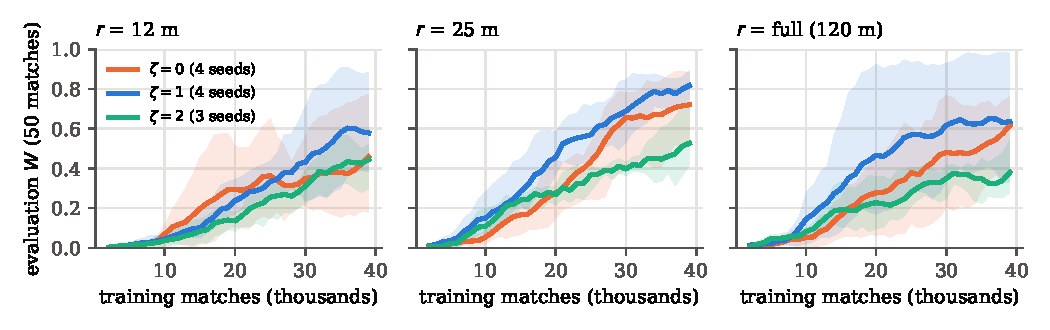
\includegraphics[width=\linewidth]{q1_curves.pdf}
  \caption{Q1 learning curves: evaluation $W$ against the full-strength opponent (50 matches every 1{,}000 training
  matches, 3-point moving average); lines are means over seeds, shading the range of the seeds.}
  \label{fig:q1curves}
\end{figure}

\textbf{More vision is not always better.} The highest scores came at 25\,m ($W$ 0.76 and 0.82 for $\zeta=0,1$), not
with full vision (0.63 and 0.68), although the seed spread is too large to call this a tested difference. At 12\,m and
25\,m the teams learned to defend deep and win the ball by tackling; 78--87\% of their goals started in their own third,
83--93\% involved two or more passes, and the median goal came 32--38 steps after winning the ball. Full-vision teams
kept the ball longer (24--32\% possession against 13--20\%), and fewer of their goals came from passing moves (46--55\%
with two or more passes, against 83--93\%). Several settings were still improving at 40{,}000 matches (Figure~\ref{fig:q1curves}).

\textbf{Learning copes with limited vision far better than rules.} The scripted team placed in our seat falls from
$W=0.45$ at 25\,m to $0.07$ at 12\,m; the learned teams fall from about 0.8 to 0.45--0.61
(Table~\ref{tab:q1}). All teams overfit to their training opponents: against the never-seen 1-2-2 they score
$W=0.01$--$0.24$, while a team trained against 1-2-2 beats it in 99\% of matches.

\begin{figure}[t]
  \centering
  \begin{minipage}[c]{0.46\linewidth}
  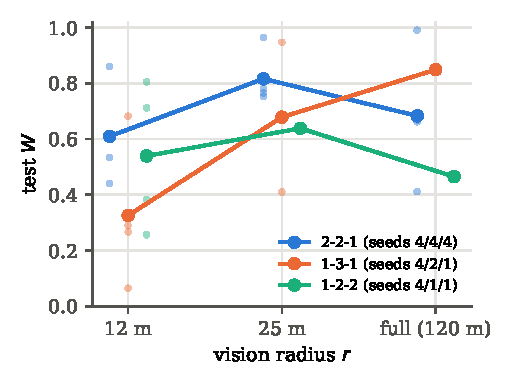
\includegraphics[width=\linewidth]{q1_formations.pdf}
  \end{minipage}\hfill
  \begin{minipage}[c]{0.51\linewidth}
  \caption{Our three formations by radius at $\zeta=1$ (small dots: seeds; the number of seeds per radius is in the
  legend). In single runs 1-2-2 was best at 12\,m (0.80) and 1-3-1 at 25\,m (0.95) and with full vision. With 4 seeds
  at 12\,m and a second 1-3-1 seed at 25\,m (0.41) this pattern disappeared: 2-2-1 has the highest mean at 12\,m and
  25\,m, but no difference between formations excludes 0.}
  \label{fig:q1form}
  \end{minipage}
\end{figure}

\textbf{The best formation does not measurably depend on the radius} (Figure~\ref{fig:q1form}). In single runs the
order flipped with $r$, so we trained three more seeds of 1-3-1 and 1-2-2 at 12\,m, where the gap was largest, and a
second 1-3-1 seed at 25\,m. The flip did not survive. At 12\,m, 2-2-1 (0.61) leads 1-2-2 (0.54; seeds 0.80, 0.71, 0.38,
0.26) by $+0.07\pm0.40$ and 1-3-1 (0.33; seeds 0.68, 0.29, 0.27, 0.07) by $+0.28\pm0.40$; at 25\,m it leads 1-3-1 by
$+0.14\pm3.31$ (two seeds). Interestingly, the scripted ranking of Phase~0 (1-3-1 best on average) does not carry over
to learned teams: 1-3-1 has the lowest learned mean at 12\,m, although not by a tested margin.

\textbf{Answer to Q1.} Within our budget a formation does not make the team measurably better at any radius, enforcing
it slightly hurts if anything, and the best formation does not measurably depend on the radius. The team finds a
workable shape by itself; with $\zeta=0$ it still stands at a similar depth and spread as with $\zeta=1$. The most robust
finding is the size of the seed effect.

%====================================================================================================================
\subsection{Results for Q2: inferring and adapting to a formation change}
\label{sec:q2}

\textbf{Design.} The opponent starts in 2-2-1 and switches once to \textbf{1-2-2}, a formation the general team never trained against (it scores
$W=0.04$ against it), at a random step between 100 and 1{,}100. In a second test it switches \emph{on
the score} (to 1-2-2 when behind, to 3-1-1 when ahead, checked every 50 steps). Teams (all play the same 300 test
matches, seeds never used in training or tuning):
\begin{itemize}[leftmargin=1.5em]
\item \textbf{keep}: the general team (trained against the four training formations) plays the whole match;
\item \textbf{oracle}: at the moment of the switch, a \emph{specialist} trained against 1-2-2 takes over; the best that
identify-then-act can do;
\item \textbf{guess}: the specialist takes over while a Bayesian filter believes the opponent is in 1-2-2;
\item \textbf{guess (no player IDs)}: the same filter without knowing which opponent is which player;
\item \textbf{GRU} and \textbf{MLP}: one policy trained end to end on exactly this switch, with and without memory
(3 seeds each at $r=25$, one at $r=12$).
\end{itemize}
The general team and the specialist are deliberately moderate checkpoints of equal strength ($W\approx0.75$ at $r=25$):
a fully trained specialist wins even after a late handover, which would hide the cost of a slow guess. The GRU and MLP
are fully trained, so their $W$ is not comparable with the pair; for them the meaningful numbers are what they lose at
the switch and how they compare with each other.

\textbf{The filter.} Position maps counted on 400 practice matches give, for each formation and ball state, how often
each opponent player stands in each 10\,m box. Each step the filter allows a switch with hazard $h$, multiplies in the
likelihood of what our five players currently see, raised to a power $\beta<1$ (consecutive steps show nearly the same
picture), and commits to the formation that leads. $\beta=0.1$ and $h=10^{-4}$ were tuned on 200 practice switch
matches from the training distribution, never on test matches. The detection delay (Eq.~\ref{eq:delay}) is the number
of steps from the switch until the guess is right (with persistence $m=1$), and regret is
$\mathrm{Reg}=W(\text{oracle})-W(\text{team})$, paired over matches.

\begin{table}[t]
\caption{Q2 switch tests (300 matches each, same seeds for every team). Regret is paired over matches against the
oracle, with a 95\% interval. Delay: median steps from the switch to a correct guess. The GRU and MLP are fully trained
teams (seed 0), not comparable in absolute $W$ with the moderate pair.}
\label{tab:q2}
\centering
\footnotesize
\setlength{\tabcolsep}{4pt}
\begin{tabular}{llcccccc}
\toprule
 & & \multicolumn{3}{c}{$r=25$\,m} & \multicolumn{3}{c}{$r=12$\,m} \\
\cmidrule(lr){3-5}\cmidrule(lr){6-8}
switch & team & $W$ & regret & delay / false al. & $W$ & regret & delay / false al. \\
\midrule
\multirow{6}{*}{random time}
 & keep general team & 0.46 & $+0.29\pm0.05$ & -- & 0.25 & $+0.28\pm0.05$ & -- \\
 & oracle & 0.75 & -- & -- & 0.53 & -- & -- \\
 & \textbf{guess} & \textbf{0.74} & $\mathbf{+0.01\pm0.04}$ & 28 / 0\% & \textbf{0.46} & $+0.07\pm0.06$ & 36 / 0\% \\
 & guess, no player IDs & 0.68 & $+0.07\pm0.05$ & 68 / 23\% & 0.39 & $+0.14\pm0.07$ & 66 / 59\% \\
 & GRU (end to end) & 0.96 & & & 0.24 & & \\
 & MLP (end to end) & 0.99 & & & 0.78 & & \\
\midrule
\multirow{6}{*}{on the score}
 & keep general team & 0.31 & $+0.44\pm0.06$ & -- & 0.23 & $+0.22\pm0.06$ & -- \\
 & oracle & 0.75 & -- & -- & 0.45 & -- & -- \\
 & \textbf{guess} & \textbf{0.73} & $\mathbf{+0.01\pm0.04}$ & 33 / 12\% & \textbf{0.39} & $+0.07\pm0.06$ & 38 / 37\% \\
 & guess, no player IDs & 0.63 & $+0.12\pm0.05$ & 61 / 43\% & 0.30 & $+0.14\pm0.06$ & 82 / 79\% \\
 & GRU (end to end) & 0.83 & & & 0.23 & & \\
 & MLP (end to end) & 0.93 & & & 0.67 & & \\
\bottomrule
\end{tabular}
\end{table}

\begin{figure}[t]
  \centering
  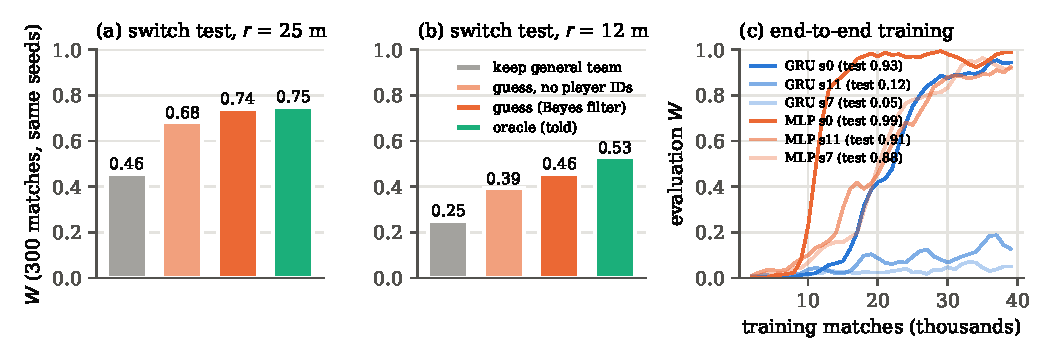
\includegraphics[width=\linewidth]{q2.pdf}
  \caption{Q2. (a, b) $W$ in matches where the opponent switches to 1-2-2 at a random time. (c) Training curves of the
  end-to-end teams at $r=25$: only one of three GRU seeds learned to win; all three MLP seeds did.}
  \label{fig:q2}
\end{figure}

\textbf{Identification is fast and almost free} (Table~\ref{tab:q2}, Figure~\ref{fig:q2}). At $r=25$ the filter finds
every switch, with a median delay of 28 steps (2.3\% of a match) and no false alarm. Handing over on the guess scores
$W=0.74$ against the oracle's 0.75 (regret $0.01\pm0.04$), i.e.\ it keeps $(0.74-0.46)/(0.75-0.46)=97\%$ of the gain
of knowing the switch; not switching costs 0.29. The delay is about the time the opponent needs to walk to its new
spots. On the score-triggered switch, which also uses 3-1-1, the guess still loses only $0.01\pm0.04$.

\textbf{Vision and player identity matter for identification.} At $r=12$ the guess loses $0.07\pm0.06$ (it keeps 75\% of
the oracle's gain), and without player IDs the filter must recognise the shape alone: delay 68 steps and false alarms in
23\% of matches at $r=25$, regret $0.14$ at $r=12$.

\textbf{End-to-end training learns robustness, not identification.} Trained on the switch, the GRU (seed 0) loses
nothing at it: its goal-difference rate per 100 steps is $+0.19$ before and $+0.26$ after the switch. A linear read-out
of its hidden state reacts quickly (first says ``1-2-2'' a median of 9 steps after the switch) but also says ``1-2-2''
\emph{before} the switch in 89\% of matches, so the memory does not track the formation in a usable way. Memory brought
no advantage: the memoryless MLP did at least as well, and training with memory was less reliable. Only 1 of 3 GRU
seeds learned to win (test $W$ 0.93, 0.12, 0.05) against all 3 MLP seeds (0.99, 0.91, 0.88); with three seeds the
difference of means, $-0.56\pm1.21$, is not distinguishable from 0, but the pattern repeats at $r=12$ (GRU 0.21, MLP
0.77, one seed each). The failed GRU seeds kept normal entropy and KL; they never found a way to beat the
full-strength opponent.

\textbf{Robustness is narrower than identification.} On the score-triggered switch, an opponent behaviour they never met
in training, the end-to-end teams drop (GRU $0.96\to0.83$, MLP $0.99\to0.93$), while identify-then-act loses nothing.
\textbf{Adaptation lag.} Aligned at the switch, the oracle and the guess need about 220--230 steps to return to their
pre-switch goal-difference rate, because a specialist that comes on mid-match takes time to settle.

\textbf{Answer to Q2.} A formation change can be identified within about 30 steps from what the players see, and acting
on the guess keeps almost all of the value of knowing it; smaller vision and missing player identities make it slower
and less reliable. End-to-end training does not learn to identify the switch; it learns a policy that is robust to both
formations, which here is even more effective but generalises less to new switching behaviour.

%====================================================================================================================
\subsection{Results for Q3: adapting to an opponent playmaker}
\label{sec:q3}

\textbf{The playmaker.} The proposal's playmaker (one opponent with full-pitch vision, otherwise unchanged) made almost
no difference to our best Q1 team, the \emph{unaware} team (\,$\zeta=0$, $r=25$, seed 0; $W$ 0.82--0.90 without a
playmaker): in the first screen (300 matches per case) only player 4 in 2-2-1 cost it anything ($W$ $0.88\to0.66$), and
with full vision plus teammates looking for the playmaker it still won all seven midfield cases ($W$ 0.55--0.90). Since a playmaker that costs
nothing cannot be adapted to, we strengthened it step by step and screened each step against the unaware team, until it
lost every midfield case. The final playmaker sees the whole pitch, its teammates prefer passing to it, it leaves its zone
to show for the ball, and its control rating is 4 everywhere (others: 0.5--1), so it wins most tackles, passes without
aiming error and scores open shots from inside 35\,m. A version whose passes were also faster was rejected because it
was identified trivially (within about 25 steps). The playmaker is therefore \emph{calibrated against the unaware team},
and its costs are large by design. Only midfielders are playmakers: seven cases (2-2-1 players 3, 4; 2-1-2 player 3;
1-3-1 players 2, 3, 4; 3-1-1 player 4), plus matches without a playmaker. Radius 25 only.

\textbf{Teams.} \emph{Unaware}: the team above. \emph{Specialists}: trained like it, but against the playmaker (one for
player 2, one for player 4; the player 3 specialist stayed below the unaware team, test $W$ 0.25, and was dropped).
\emph{Oracle}: the right specialist from kick-off (unaware team if there is none). \emph{Adaptive}
(identify-then-act): the unaware team until a Bayesian filter commits, then the specialist for its guess. The filter
pools, for each opponent number, how far it stands from the ball (7 distance bins, or unseen) in each ball state; maps
come from 100 practice matches per case, and $\beta=0.05$ and the commit threshold 0.95 were tuned on 50 other matches
per case. \emph{Mix}: a single GRU trained on all 24 cases (4 formations $\times$ no playmaker or player 1--5), drawn per
match, not told who the playmaker is; \emph{mix-told} is told; \emph{mix-no-shadow} lacks the \textsc{shadow} action.
Every team plays the same 500 matches per case (seeds never used before), so all comparisons are paired.

As in Eq.~\eqref{eq:q3}, the cost is $E=W(\text{unaware, no playmaker})-W(\text{unaware, playmaker})$, the recovery
is $\kappa=(W(\text{team})-W(\text{unaware}))/E$ ($\kappa=1$: all of the cost won back), and the regret is
$W(\text{oracle})-W(\text{adaptive})$.

\begin{table}[t]
\caption{Q3 in the four cases with a specialist (500 matches per case, same seeds for every team). $E$ has a 95\%
interval of about $\pm0.05$, so $\kappa$ is defined in every case. Single training run per team.}
\label{tab:q3}
\centering
\small
\begin{tabular}{lcccccccc}
\toprule
case & \multicolumn{4}{c}{$W$} & cost & \multicolumn{3}{c}{recovery $\kappa$} \\
\cmidrule(lr){2-5}\cmidrule(lr){7-9}
 & unaware & adaptive & oracle & mix & $E$ & adaptive & oracle & mix \\
\midrule
1-3-1, player 2 & 0.22 & 0.50 & 0.71 & 0.68 & 0.60 & 0.47 & 0.81 & 0.77 \\
3-1-1, player 4 & 0.36 & 0.56 & 0.64 & 0.65 & 0.54 & 0.36 & 0.52 & 0.53 \\
2-2-1, player 4 & 0.21 & 0.32 & 0.46 & 0.74 & 0.65 & 0.17 & 0.38 & 0.81 \\
1-3-1, player 4 & 0.02 & 0.04 & 0.12 & 0.54 & 0.80 & 0.02 & 0.12 & 0.64 \\
\midrule
no playmaker (4 formations, mean) & 0.85 & 0.81 & 0.85 & 0.72 & & & & \\
\bottomrule
\end{tabular}
\end{table}

\begin{figure}[t]
  \centering
  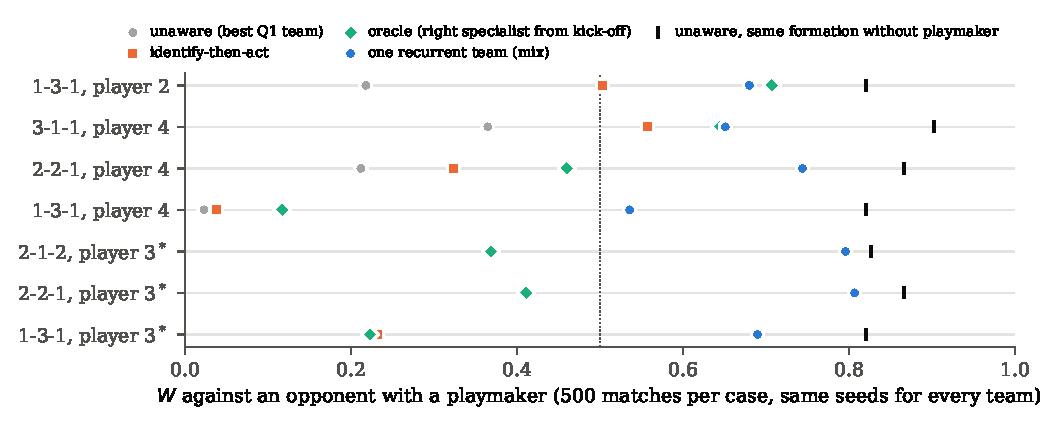
\includegraphics[width=\linewidth]{q3.pdf}
  \caption{Q3: $W$ of each team in every playmaker case (500 matches per case). The black tick is the unaware team in
  the same formation without a playmaker, so its distance to the grey dot is the cost $E$. $^*$Player 3 has no
  specialist, so the adaptive team and the oracle play as the unaware team there.}
  \label{fig:q3}
\end{figure}

\textbf{The playmaker costs the unaware team a lot} (Table~\ref{tab:q3}, Figure~\ref{fig:q3}): $E$ = 0.54--0.80 in
the four specialist cases and 0.46--0.60 in the three player-3 cases, every interval excluding zero by a wide margin. The
specialists turn two losing cases into winning ones (oracle $W$ 0.71 and 0.64).

\textbf{The playmaker can be identified from behaviour, but slowly.} From positions relative to the ball alone, the
filter's committed guess is right in 100\%, 100\% and 99\% of matches for 1-3-1 player 2, 3-1-1 player 4 and 2-2-1
player 4, at a median step of 141, 169 and 194. For 1-3-1 player 4 it is right in only 68\% (median step 507).
Without a playmaker the filter wrongly names one in 12--38\% of matches.

\textbf{Identify-then-act recovers part of the cost and stays below the oracle}, as hypothesised: $\kappa$ 0.02--0.47
against the oracle's 0.12--0.81, regret 0.08--0.20. Over the four specialist cases the adaptive team beats the unaware
team by $+0.15\pm0.02$ and the oracle beats the adaptive team by $+0.13\pm0.02$ (paired). In the three easy cases almost
all of the regret comes from the steps the unaware team plays before the commit: even a commit before step 150 costs
0.06--0.25 in $W$. Where the specialist itself is weak (1-3-1 player 4, oracle 0.12), identification cannot help.
False alarms are expensive because the specialists play poorly against ordinary teams ($W$ 0.11--0.60 without a
playmaker): when the filter wrongly names player 4 in a 2-2-1 match, $W$ in those matches falls from 0.63 to 0.23, and
over all no-playmaker matches the adaptive team loses 0.04 on average.

\textbf{The specialists do not neutralise the playmaker by marking it.} About one in four of their \textsc{shadow}
steps is on the playmaker (21--34\%), no more than for the unaware team (19--33\%) and close to the 20\% of picking an
opponent at random. Whatever the specialists do differently, it is not man-marking.

\textbf{One recurrent team for every case does best.} Trained from scratch, the three mix teams did not learn: with
every case drawn per match they rarely won often enough for the easy start to make the opponent harder, and after
13{,}000--29{,}000 matches their test $W$ was 0.01--0.02. We therefore \emph{warm-started} all three from the Q2 GRU seed 0
(same observation and actions; test $W$ 0.93 against the full-strength opponent), with a fresh optimiser and the easy
start from the beginning, and trained them for 15{,}000 matches. Mix-told's six extra inputs start at weight 0, so all
three start identical and only training separates them. Over the seven playmaker cases mix averages $W=0.70$, against
0.35 for identify-then-act and 0.42 for the oracle of specialists; paired over the same 3{,}500 matches, mix beats
adaptive by $+0.35\pm0.02$ and the oracle by $+0.28\pm0.02$, and its recovery $\kappa$ is 0.53--0.81. Without a
playmaker it is worse than the unaware team (0.72 against 0.85). This comparison mixes the method with a better start:
the mix teams began from a team that could already play, while the specialists trained from scratch.
Among the mix teams the comparison is fair: being told who the playmaker is adds $+0.05\pm0.02$ over the playmaker
cases ($+0.02\pm0.01$ over all 11 cases), and the team \emph{without} \textsc{shadow} scores higher than mix in every
case ($+0.15\pm0.01$ over all 11), so the shadow action is not needed, in line with the marking result above. These
intervals are over matches with one training run per team; they show that these teams differ, not that every training
run would.

\textbf{Answer to Q3.} A playmaker with real abilities costs the unaware team the match. It can be identified from
behaviour in most cases, but only after 140--200 steps. Identify-then-act recovers 2--47\% of the cost and stays below
the oracle (12--81\%), limited mostly by the specialists and then by the delay. A single recurrent team trained over all
cases, warm-started from a trained team, recovers the most (53--81\%) without identifying the playmaker explicitly.

%====================================================================================================================
\section{Discussion}
\label{sec:discussion}

\begin{table}[t]
\caption{The hypotheses of our proposal and what the data say (all at the stated budget).}
\label{tab:hyp}
\centering
\small
\begin{tabular}{p{0.46\linewidth}p{0.47\linewidth}}
\toprule
Hypothesis (proposal) & Outcome \\
\midrule
Q1: structure helps more at small radii & \no: point estimates lean that way ($+0.16$ at 12\,m vs.\ $+0.05$), all intervals include 0 \\
Q1: knowing the anchor ($\zeta=1$) captures most of the benefit & no benefit to capture; enforcing ($\zeta=2$) is lowest at 25\,m and full vision (not tested significant) \\
Q1: the best formation changes with $r$ & \no: an apparent flip in single runs vanished with 4 seeds \\
Q2: recurrent beats memoryless & \no: MLP at least as good; 1/3 GRU seeds vs.\ 3/3 MLP seeds learned \\
Q2: the belief filter is a strong baseline & \yes: regret $0.01\pm0.04$ at $r=25$, 28-step median delay \\
Q2: the gap to the oracle grows as $r$ shrinks & \textbf{consistent}: regret $0.07\pm0.06$ at $r=12$ (excludes 0) vs.\ $0.01\pm0.04$ at $r=25$; the difference between radii is not tested \\
Q3: the playmaker costs the unaware team measurable $W$ & \yes: $E=0.46$--$0.80$ (with a calibrated playmaker) \\
Q3: the adaptive team recovers part but stays below the oracle & \yes: $\kappa$ 0.02--0.47 vs.\ 0.12--0.81 \\
Q3: identification is easier when its play reveals it & \yes: fast passes gave it away in about 25 steps; position alone takes 140--200 \\
Q3: the cost is larger at small $r$ & not tested (radius 25 only) \\
\bottomrule
\end{tabular}
\end{table}

\textbf{Learned robustness beat both structure and explicit inference.} In Q1 the team without a formation found a
workable shape by itself; in Q2 the end-to-end teams ignored the switch and simply beat both formations; in Q3 the single
recurrent team beat the identify-then-act pipeline. Explicit identification is fast and nearly lossless in Q2, but
\emph{acting} on a guess requires good, broad specialists, and a narrow specialist turns every false alarm into a
heavy loss (Q3). Its advantage is generalisation: on a switch pattern the end-to-end teams had not seen, they dropped
while identify-then-act did not (Q2).

\textbf{More information is not automatically better.} Full vision was no better than 25\,m in Q1, and a playmaker with
only extra vision hardly mattered in Q3. Information helps when the team, or the opponent, can act on it.

\textbf{Seed variance is a result in itself.} One Q1 setting spans $W=0.18$ to 0.76 across seeds, two of three GRU
seeds failed in Q2, and the formation ``flip'' disappeared with more seeds. With one seed per setting this study would
have reported several clean but false effects. For small-budget MARL comparisons, multiple seeds and intervals over
seeds are not optional~\cite{henderson2018matters,agarwal2021precipice}.

%====================================================================================================================
\section{Limitations}
\label{sec:limitations}
\begin{itemize}[leftmargin=1.5em]
\item \textbf{Seeds and budget.} 3--4 seeds per Q1 setting give intervals of about $\pm0.15$ (25\,m) to $\pm0.45$ (12\,m);
smaller effects may exist but cannot be claimed. Several settings were still improving at 40{,}000 matches.
\item \textbf{One opponent.} All results are against one scripted opponent whose behaviour is fixed; the counter-attack
style partly exploits how it attacks. All Q1 teams fail against the never-seen 1-2-2.
\item \textbf{Q2 uses one target formation (1-2-2)} and a deliberately moderate general/specialist pair; the pair and the
filter are single runs, and the GRU result at $r=25$ rests on its one successful seed.
\item \textbf{Q3 uses one training run per team and radius 25 only.} The playmaker was calibrated against the unaware
team, so the costs are large by design. The mix teams were warm-started and trained for 15{,}000 matches, the
specialists from scratch for 40{,}000, so mix against adaptive/oracle compares methods \emph{and} starts.
\item \textbf{Best-checkpoint selection} picks the best of 40 evaluations of 50 matches, which flatters the evaluation
$W$; all reported $W$ come from new test seeds and are unbiased for the chosen checkpoint.
\item \textbf{Simplifications:} 2D ground passes only, teammates and the ball always visible, opponents identified by
number (relaxed in the ``no player IDs'' filter).
\end{itemize}

%====================================================================================================================
\section{Conclusion}
\label{sec:conclusion}
Under limited vision a formation did not make our learned team measurably better, and enforcing it slightly hurt if
anything. Identifying what the opponent is doing is possible and fast, about 30 steps for a formation change and about
150 for a playmaker, and with a good specialist acting on it keeps almost all of an oracle's value. But the strongest
teams in Q2 and Q3 did not identify anything: they learned to be robust to all the opponents they met. The answer to
``structure or information?'' in this game is therefore a third option, \emph{learned robustness}, with explicit
inference as the more general but more fragile alternative, and with the caveat that at this budget the training seed
decides more than either.

%====================================================================================================================
\section{Contribution}
\label{sec:contrib}

\begin{table}[h]
\caption{Tasks of each member.}
\label{tab:contrib}
\centering
\small
\begin{tabular}{p{0.15\linewidth}p{0.22\linewidth}p{0.55\linewidth}}
\toprule
Member & Responsibility & Tasks \\
\midrule
Arpan Gupta & Environment and opponent (\S\ref{sec:env}) & 2D environment (passing, interception, dribbling, tackling,
shooting, control rating, limited vision); zonal opponent, playmaker variant, shadow action, formation switching;
Phase~0 calibration and checks, including the formation win matrix. \\
Deep Buha & Learning and Q1 (\S\ref{sec:q1}) & Parameter-shared PPO with centralised critic (MLP and GRU); reward
design with potential-based shaping and the easy-start curriculum; structure levels and the Q1 experiments. \\
Ramji Purwar & Inference and playmaker, Q2 and Q3 (\S\ref{sec:q2}, \S\ref{sec:q3}) & Bayesian filters (tuned on
training data only), oracle and specialist teams; Q2 experiments (switch tests, delay, lag, regret); Q3 experiments
(cost, recovery, identification, shadow behaviour, ablation); evaluation pipeline with confidence intervals, tables and
figures. \\
\bottomrule
\end{tabular}
\end{table}


%Bibliography
\bibliographystyle{unsrt}
\bibliography{references}

%====================================================================================================================
\appendix

\section{Changes from the proposal}
\label{app:changes}
\begin{center}
\small
\begin{tabular}{p{0.27\linewidth}p{0.30\linewidth}p{0.35\linewidth}}
\toprule
Proposal & What was run & Why \\
\midrule
Bounded, annealed shaping with an outcome bonus & Goals $\pm100$ plus potential-based shaping, never faded & leaves the optimal policy unchanged and cannot be farmed \\
Vision limits opponents and the ball & limits opponents; ball always seen & simplification of the final game: the study varies how many opponents a player sees \\
3 radii plus full vision & 12, 25 and full (120\,m) & compute \\
3 seeds on the grid, 5 on headline settings & 4 seeds ($\zeta=0,1$), 3 ($\zeta=2$); 4 seeds for 1-3-1 and 1-2-2 at 12\,m & compute; seeds added where results disagreed \\
Opponent formation drawn over all 5 & 4 (1-2-2 held out) & 1-2-2 is far stronger; used as the Q2 target \\
Q2: belief-augmented policy & identify-then-act handover to a specialist; MLP added as memoryless baseline & isolates the value of the guess; the MLP tests whether memory is what helps \\
Q2: held-out switch times and formation pairs & held-out switch times; one target (1-2-2) & one specialist per target formation \\
Q3: playmaker = full vision only, positions 1--5 & full vision + free role + passing preference + control 4; midfielders only & vision alone cost the unaware team almost nothing \\
Q3: no-shadow ablation, one recurrent team & both run, warm-started from the Q2 GRU & from scratch they did not learn \\
Q3: small and large $r$ & radius 25 only & compute \\
\bottomrule
\end{tabular}
\end{center}

\section{Compute and runs}
\label{app:compute}
We trained 65 teams: 46 for Q1, 10 for Q2 (GRU and MLP seeds, two 1-2-2 specialists), and 9 for Q3 (three
specialists, three mix teams from scratch, three warm-started). Together they played about 2.48 million training
matches ($2.97\times10^9$ game steps, each with five player decisions). Every trained team was tested on 300 new
matches; the Q2 switch tests used 300 matches per team and test, and the Q3 comparison 500 matches per case and team
(33{,}000 matches). Runs used seven CPU servers, one run per server at a time.

\section{Reproducibility}
\label{app:repro}
All code, the results of every run (\texttt{result.json}, training logs, the checkpoints the results use) and all
evaluation files are in the project repository (\texttt{football\_adapt/runs/}). One command checks the results:
\begin{verbatim}
bash reproduce.sh          # add --full or --all for longer replays
\end{verbatim}
It runs the unit tests, recomputes every table, figure and number of this paper from the stored run files
(\texttt{runs/\_tools/final\_report.py} and \texttt{paper/make\_figs.py}, which also writes \texttt{paper/numbers.txt},
listing each number used here with the file it comes from) and compares them with the committed versions, and replays
stored teams on their recorded matches. Each run stores its training arguments, and
\texttt{python -m scripts.train\_command runs/q1/z1\_r25/s0} prints the command that trained it. The detailed
per-question reports are \texttt{docs/reportQ1.md}, \texttt{reportQ2.md} and \texttt{reportQ3.md}.

\end{document}
